\documentclass{article}

\PassOptionsToPackage{numbers,compress}{natbib}
\usepackage[dblblindworkshop]{neurips_2026}
\workshoptitle{From Pretrained Representations to Acting Agents}

\usepackage[utf8]{inputenc}
\usepackage[T1]{fontenc}
\usepackage{amsmath,amssymb}
\usepackage{booktabs}
\usepackage{float}
\usepackage{placeins}
\usepackage{needspace}
\usepackage{graphicx}
\usepackage{microtype}
\usepackage{xcolor}
\usepackage{url}
\usepackage{hyperref}

\newcommand{\lewm}{LeWM}
\newcommand{\trtwo}{TR2}
\newcommand{\curpred}[2]{#1\,/\,#2}

\title{When LeWM Misses the Color:\\Cue Binding in Tunnel Rooms}
\author{Anonymous Authors}

\begin{document}
\maketitle

% Keep natural paragraph and heading gaps when large floats constrain a page.
\raggedbottom

\begin{abstract}
A world model can learn where an object is without learning the detail that
makes it useful for action. We introduce Tunnel Rooms Color, a navigation
benchmark in which matching tunnel colors determine teleportation
destinations. Reaching an image-specified goal by the direct route requires
using color to choose the correct tunnel. We find that an adapted
LeWorldModel (LeWM) learns tunnel locations accurately but represents their
cue-dependent destinations much less reliably. Across variants, linear probes achieve
mean $R^2$ above .90 for locations but only .20--.26 for cue-indexed
coordinates;
image reconstructions blur cue distinctions; and goal-energy maps assign
low cost near both candidate tunnels in an illustrated scene. Planning is
also difficult: success on the farther correct tunnel is 16--52\% across
Color, Shape, and a green/blue palette. Controlled cue swaps change the
representation, yet predicted trajectories understate the separation between
the resulting destinations. Tunnel Rooms thus tests how visible distinctions
become useful for predicting and choosing routes.
\end{abstract}

\section{Introduction}

Joint-embedding predictive architectures (JEPAs) have become a prominent
approach to learning visual representations and world models
\citep{assran2023ijepa,bardes2024vjepa,assran2025vjepa2,murlabadia2026vjepa21}.
Their appeal is abstraction: predicting in feature space can avoid spending
capacity on pixel details that are irrelevant or difficult to predict
\citep{lecun2022path,balestriero2025lejepa}. This principle also supports
planning from learned dynamics \citep{sobal2025latentplanning,maes2026leworldmodel}.
For an acting agent, however, a visually small detail can determine which
action reaches the goal. Learning to ignore detail is useful only when the
right distinctions survive.

We investigate this tension with \emph{Tunnel Rooms Color}. Two tunnels
connect a central room to different destinations, and their colors reveal
which destination each tunnel reaches. A model can therefore learn the
room geometry, locate every tunnel, and still lack a reliable basis for
choosing between them. The environment separates these abilities with
minimal visual complexity. Shape and alternate-palette variants let us
ask whether the difficulty is specific to one choice of colors.

We study LeWorldModel (LeWM) through coordinate probes, image
reconstructions, goal-energy maps, and planning. These tests reveal a gap
between locating tunnels and recovering their cue-dependent destinations.
Controlled swaps further distinguish a response to changed cues from a
prediction of where they lead. We contribute the benchmark and this
empirical finding; its cause remains open.

\section{Tunnel Rooms: the cue determines the destination}

A central room contains two tunnel entrances, each paired with an endpoint
in a separate destination room. Entering a green tunnel teleports the agent
beside the other green endpoint; orange follows the same rule. A goal image
shows the requested agent position in a destination room. The direct route
requires matching that room's tunnel to the corresponding entrance in the
central room (Figure~\ref{fig:taskrank}).

Tunnel positions and color assignments vary across episodes. Knowing which
entrance is higher, lower, or nearer is therefore different from knowing
where it leads. We call the association between a tunnel's cue and its
paired destination \emph{cue binding}. A scripted agent that knows the
pairings collects successful trajectories, so the training data contain
examples of cue-guided routes. Exploratory behavior may still reach the
goal without using the cue; our evaluation distinguishes cases where the
correct tunnel is nearer from those where it is farther away.

We consider three renderings of the same trajectories. \emph{Color} uses
green and orange markers. \emph{Shape} replaces them with triangles and
diamonds, while \emph{Palette} uses green and blue. These changes preserve
the underlying positions, actions, and teleportation pairings. We train LeWM
from scratch on 10,000 trajectories per rendering. It predicts the next
latent state from an observation history and an action sequence. Our primary
model uses spatial features and an auxiliary inverse-dynamics loss, which
predicts actions from consecutive states. Appendix~\ref{app:ablations}
compares both additions with the native model.

\begin{figure}[t]
  \centering
  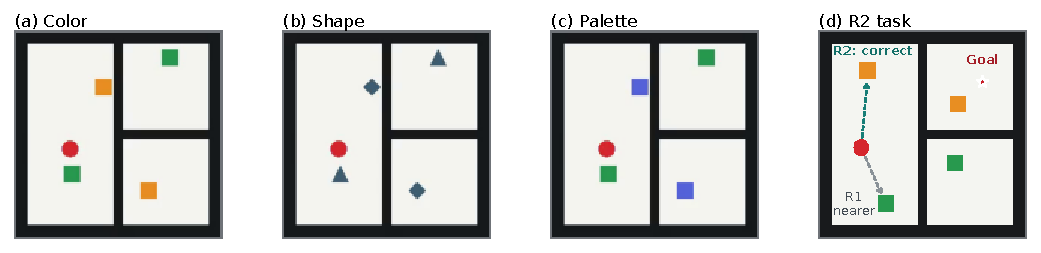
\includegraphics[width=\linewidth]{figures/tunnel_variants_and_rank.pdf}
  \caption{\textbf{The same geometry supports different cue-guided routes.}
  (a--c) Color, Shape, and Palette renderings of one trajectory.
  Matching cues identify paired tunnels. (d) An R2 task: the entrance leading
  to the goal room is farther from the agent than the other entrance.
  R1/R2 rank the correct entrance; they are not fixed tunnel identities.}
  \label{fig:taskrank}
\end{figure}

\section{LeWM learns locations more reliably than cues}

We first ask what LeWM's representation makes accessible. We freeze the
model and fit identical linear probes to predict the same four tunnel
endpoints in two ways: by their top/bottom positions, or by their color or
shape identities. Both tasks recover coordinates; only the second requires
binding the cue to the correct endpoint. Mean absolute error (MAE) measures
coordinate error in pixels, and $R^2$ measures explained variance.

The contrast is substantial (Table~\ref{tab:probes}). Averaging the four endpoints on
Color gives location MAE of 3.83 pixels and $R^2=.934$, versus cue MAE of
27.40 pixels and $R^2=.224$. The cue error is only modestly below
the constant cue predictor's 31.19 pixels. Shape and Palette show the same ordering.
The representation thus supports accurate localization much more readily
than cue-conditioned localization. The probes test accessibility to a
linear readout, not the complete absence of cue information. A small MLP
also leaves a wide location--cue gap (Appendix~\ref{app:nonlinear}).
Appendix~\ref{app:ablations} reports controls for the model adaptations
and additional palette conditions.

\begin{table}[!htbp]
\centering
\caption{\textbf{The location--cue gap holds across individual endpoints.}
MAE (pixels) and $R^2$ from frozen representations, averaging $x/y$ scores
for each endpoint. Top/bottom are ordered independently in the central
room and destination rooms; same-cue rows identify paired endpoints.}
\label{tab:probes}
\renewcommand{\arraystretch}{1.10}
\setlength{\tabcolsep}{4pt}
\begin{tabular*}{\linewidth}{@{\extracolsep{\fill}}llrrrr@{}}
\toprule
 & & \multicolumn{2}{c}{Central room} & \multicolumn{2}{c}{Destination rooms} \\
\cmidrule(lr){3-4}\cmidrule(l){5-6}
Variant & Endpoint label & MAE $\downarrow$ & $R^2\uparrow$ & MAE $\downarrow$ & $R^2\uparrow$ \\
\midrule
Color & Top & 4.63 & .919 & 2.72 & .960 \\
 & Bottom & 5.14 & .900 & 2.82 & .958 \\
 & Green & 25.05 & .256 & 29.81 & .180 \\
 & Orange & 25.01 & .289 & 29.72 & .172 \\
\midrule
Shape & Top & 5.88 & .868 & 3.19 & .941 \\
 & Bottom & 6.06 & .872 & 3.14 & .948 \\
 & Triangle & 25.18 & .229 & 30.75 & .144 \\
 & Diamond & 25.80 & .253 & 30.47 & .184 \\
\midrule
Palette & Top & 4.79 & .913 & 2.63 & .962 \\
 & Bottom & 5.34 & .893 & 2.96 & .952 \\
 & Green & 24.93 & .262 & 29.06 & .217 \\
 & Blue & 24.95 & .315 & 28.88 & .239 \\
\bottomrule
\end{tabular*}
\end{table}

Image reconstructions make the difficulty visible. A separate decoder
learns to reconstruct observations from LeWM's representation without
letting reconstruction change that representation. The decoded images
retain the room layout, but tunnel colors become mixed and shape markers
become faint (Figure~\ref{fig:decoders}). Reconstruction can blur distinctions
because of uncertainty or limitations of the decoder itself
\citep{mathieu2016video}. These images complement the coordinate probes:
both suggest that the scene's broad structure is easier to recover than
the cues that distinguish routes.

\begin{figure}[t]
  \centering
  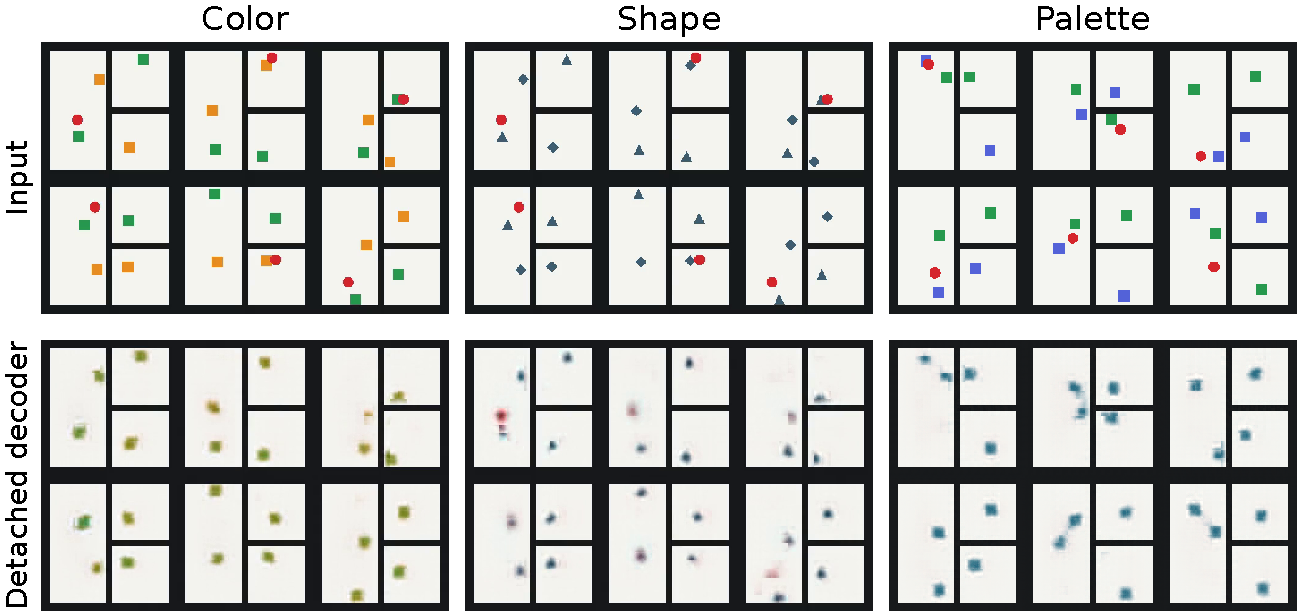
\includegraphics[width=\linewidth]{figures/lewm_spatial_three_cue_decoders.pdf}
  \caption{\textbf{Reconstructions preserve the rooms but weaken their cues.}
  Original observations (top) and decoded images (bottom) for Color, Shape,
  and Palette. All six recorded clips per variant are shown. Snapshot
  timing and the decoder protocol are given in
  Appendix~\ref{app:planning}.}
  \label{fig:decoders}
\end{figure}

\section{From cues to predicted destinations}

A cue must do more than change an image representation: it must distinguish
routes to a goal. We first compare each observed state's representation
with a fixed goal image while moving the agent through the rooms.
Lower \emph{goal energy} means greater similarity to that goal; this static
map does not use the dynamics predictor.

Figure~\ref{fig:similarity} contrasts these maps with an approximate geodesic
reference through the true paired tunnels. Switching the goal room changes
which entrance the reference favors. LeWM retains broad low-energy regions
near both entrances and destination endpoints. The maps do change with the
goal, but distinguish the routes less clearly in this scene. The reference
illustrates a routing distinction; it does not prescribe latent energy values.
Appendix~\ref{app:landscapes} gives the sampling procedure and further maps.

\begin{figure}[!t]
  \centering
  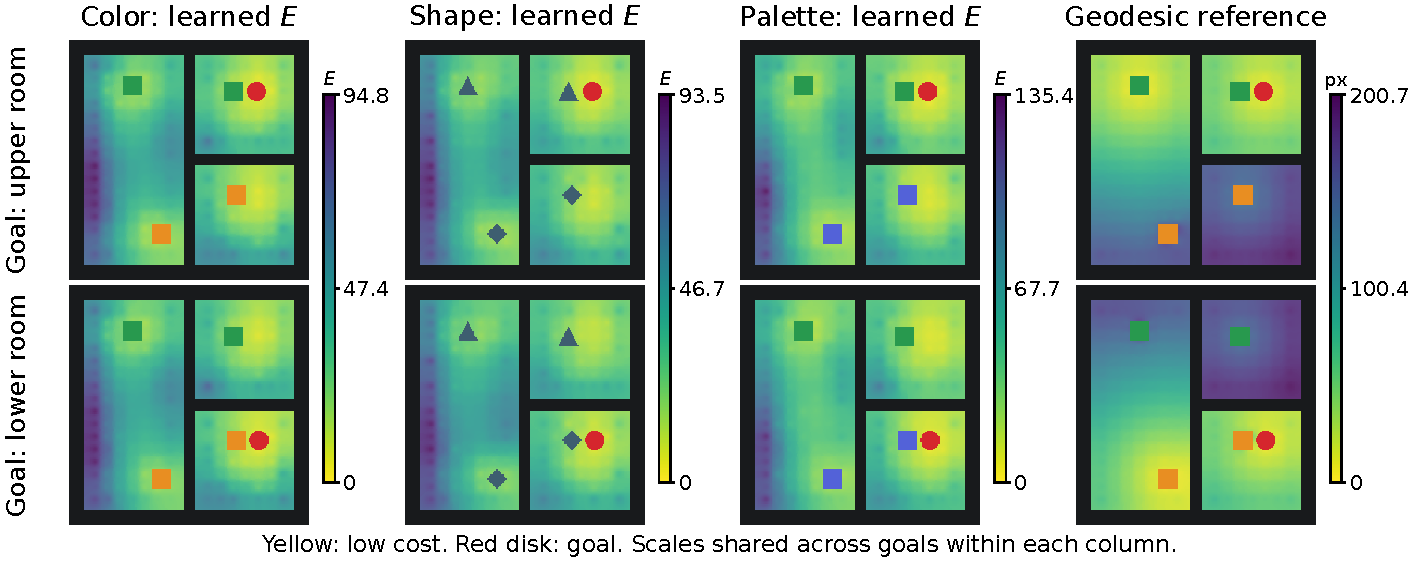
\includegraphics[width=\linewidth]{figures/lewm_spatial_three_cue_goal_distance.pdf}
  \caption{\textbf{The correct route changes with the goal; LeWM's low-energy regions remain broad.}
  Left: LeWM goal energies for Color, Shape, and Palette. Right: geodesic travel
  distance through the true paired tunnels. Rows change the goal (red disk);
  yellow denotes low cost. Each column shares a scale across goals.
  Latent energy and travel distance have different units.}
  \label{fig:similarity}
\end{figure}

We then exchange the two central-room cues, keeping the unordered portal
locations fixed and changing which destination each entrance reaches.
The encoder responds to this swap. Under identical actions, however, the
observed states separate further after teleportation while open-loop predictions
understate that separation (Appendix~\ref{app:portal-swap}). This tests a
cue's consequences more directly, although general rollout error may also
contribute.

\Needspace{8\baselineskip}
We rank the two central-room entrances by distance from the initial agent
position. In R1 tasks, the nearer entrance leads to the goal room; in R2
tasks, the agent must choose the farther entrance instead. These ranks
describe tasks, not fixed colors or tunnel positions. Both cross-entropy
method (CEM) and gradient-descent (GD) planning are less successful on R2
across all variants (Table~\ref{tab:rankplanning}). On Color, CEM success
falls from 80\% to 16\%, and GD from 64\% to 52\%. Longer routes may themselves
be harder to plan, so this contrast does not isolate cue binding as the
cause. Appendix~\ref{app:planning} gives the full protocol.

\begin{table}[!htbp]
\centering
\caption{\textbf{Planning is less successful when the correct tunnel is farther away.}
LeWM success over 25 episodes per rank, using the checkpoints evaluated by
the linear probes. R1: the nearer entrance reaches the goal room; R2: the
farther entrance does. CEM: cross-entropy method; GD: gradient descent.}
\label{tab:rankplanning}
\renewcommand{\arraystretch}{1.12}
\begin{tabular*}{\linewidth}{@{\extracolsep{\fill}}lrrrr@{}}
\toprule
Variant & CEM R1 $\uparrow$ & CEM R2 $\uparrow$ & GD R1 $\uparrow$ & GD R2 $\uparrow$ \\
\midrule
Color & 80\% & 16\% & 64\% & 52\% \\
Shape & 88\% & 24\% & 76\% & 40\% \\
Palette & 80\% & 28\% & 84\% & 32\% \\
\bottomrule
\end{tabular*}
\end{table}

\section{Discussion and conclusion}

Tunnel Rooms separates locating an entrance from knowing where it leads.
LeWM's linear and nonlinear probes recover location more reliably than cue
binding. The encoder detects controlled cue swaps, but predicted rollouts
understate their consequences after teleportation. Planning is also less
successful when reaching the goal requires choosing the farther entrance.

One possible explanation is limited exposure to crossings that reveal cue
binding. Increasing crossing-related training windows produces brighter
reconstructions without consistent gains in cue MAE or $R^2$; the result is
inconclusive (Appendix~\ref{app:exposure}). Further work should separate cue
binding from general prediction error, hold training effort fixed in exposure
ablations, and replicate these findings across runs and environments.

\clearpage

% Compact reference entries without changing the body font or page geometry.
\setlength{\bibsep}{2pt}
\bibliographystyle{abbrvnat}
\bibliography{references}

\appendix

\section{Inverse dynamics modeling loss}
\label{app:ablations}

We add inverse dynamics to improve agent localization and planning, while
leaving cue binding unsupervised.

\subsection{Predictive and inverse-dynamics objectives}

We train randomly initialized ViT-tiny models on 10,000 successful
trajectories for ten epochs, with batch size 128 and seed 3072. For a
192-dimensional projected state $z_t$ and its prediction $\hat z_{t+1}$,
\[
\mathcal L=\mathcal L_{\mathrm{pred}}+.09\mathcal L_{\mathrm{SIGReg}}
+\lambda_{\mathrm{IDM}}\mathcal L_{\mathrm{IDM}},\qquad
\mathcal L_{\mathrm{pred}}=\frac{1}{192}\mathbb E\|\hat z_{t+1}-z_{t+1}\|_2^2,
\]
\[
\mathcal L_{\mathrm{IDM}}=\frac{1}{10}\mathbb E\|h([z_{t+1},z_t])-a_t\|_2^2.
\]
SIGReg encourages isotropic Gaussian states. The target $a_t$ contains five
normalized 2-D actions. The training-only inverse head is
Linear$(384,512)$, LayerNorm, GELU, and Linear$(512,10)$; its gradients pass
through both states. We use $\lambda_{\mathrm{IDM}}=3.125$, versus zero for
the predictive objective without IDM. The zero-weight controls retain the
same inverse head but disable its loss. Inverse dynamics and auxiliary-task theory motivate
preserving action-relevant features
\citep{ivashkov2026sensorimotor,yu2025auxjepa}; our head receives no cue or
portal-pairing labels.

\subsection{Agent localization and planning}

Adding IDM improves agent-position probes (Table~\ref{tab:agentidm}) and
planning (Table~\ref{tab:idmplanning}). With spatial aggregation, pooled
CEM/GD success rises from 8/8\% to 48/58\%; with CLS, it rises from 4/8\%
to 38/40\%. Within each readout, initialization, training budget, and
evaluation are matched, and only the IDM weight changes.

\begin{table}[!htbp]
\centering
\caption{\textbf{IDM makes the agent's position more accessible.}
Linear probes of agent coordinates on the same four Color checkpoints as
Table~\ref{tab:idmplanning}. Current and predicted states target the current
and next agent position, respectively; MAE is in pixels and $R^2$ averages
$x/y$ scores. Probes fit on 640 episodes and evaluate on 256 disjoint episodes.}
\label{tab:agentidm}
\renewcommand{\arraystretch}{1.12}
\begin{tabular*}{\linewidth}{@{\extracolsep{\fill}}llrrrr@{}}
\toprule
Readout & IDM weight & \multicolumn{2}{c}{Current state} & \multicolumn{2}{c}{Predicted state} \\
\cmidrule(lr){3-4}\cmidrule(l){5-6}
 & & MAE $\downarrow$ & $R^2\uparrow$ & MAE $\downarrow$ & $R^2\uparrow$ \\
\midrule
CLS & 0 & 44.68 & -.068 & 46.11 & -.077 \\
CLS & 3.125 & 16.78 & .703 & 26.21 & .493 \\
Spatial $8\times8$ & 0 & 45.70 & -.189 & 44.77 & -.103 \\
Spatial $8\times8$ & 3.125 & 20.87 & .680 & 25.28 & .537 \\
\bottomrule
\end{tabular*}
\end{table}

\begin{table}[!htbp]
\centering
\caption{\textbf{IDM improves planning with either readout.}
Color task success (\%); every cell reports CEM/GD. R1/R2 have 25 cases
each; Cue 1 (green) and Cue 2 (orange) have 16/34 cases, pooling ranks.
Within each readout, the IDM pair shares initialization, training budget,
and evaluation settings.}
\label{tab:idmplanning}
\renewcommand{\arraystretch}{1.12}
\setlength{\tabcolsep}{3pt}
\begin{tabular*}{\linewidth}{@{\extracolsep{\fill}}llcccc@{}}
\toprule
Readout & IDM weight & \multicolumn{2}{c}{Rank-based performance $\uparrow$} & \multicolumn{2}{c}{Cue-based performance $\uparrow$} \\
\cmidrule(lr){3-4}\cmidrule(l){5-6}
 & & R1 & R2 & Cue 1 & Cue 2 \\
\midrule
CLS & 0 & 8/12 & 0/4 & 12.5/12.5 & 0.0/5.9 \\
CLS & 3.125 & 68/52 & 8/28 & 50.0/50.0 & 32.4/35.3 \\
Spatial $8\times8$ & 0 & 12/12 & 4/4 & 12.5/6.3 & 5.9/8.8 \\
Spatial $8\times8$ & 3.125 & 80/64 & 16/52 & 56.3/62.5 & 44.1/55.9 \\
\bottomrule
\end{tabular*}
\end{table}

\FloatBarrier
\section{Spatial aggregation}
\label{app:aggregator}

Replacing CLS with spatial aggregation improves tunnel localization under
both objectives (Table~\ref{tab:readoutcontrols}). With IDM, tunnel MAE
falls from 7.42 to 3.83 pixels and $R^2$ rises from .684 to .934. This gain
concerns tunnel positions: agent-position probes are stronger with CLS+IDM
(Table~\ref{tab:agentidm}). Readout comparisons share the seed and budget,
but encoder initialization differs because constructing the aggregator
consumes random numbers.

\begin{table}[ht]
\centering
\caption{\textbf{Spatial aggregation improves tunnel localization at either IDM weight.}
Current projected states from the same four epoch-10 Color checkpoints as
Tables~\ref{tab:agentidm} and \ref{tab:idmplanning}, all trained with the same
implementation and seed 3072. MAE and $R^2$ use the same four tunnel endpoints,
indexed by cue or position; agent coordinates are evaluated separately.}
\label{tab:readoutcontrols}
\renewcommand{\arraystretch}{1.12}
\begin{tabular*}{\linewidth}{@{\extracolsep{\fill}}llrrrr@{}}
\toprule
Readout & IDM weight & Cue MAE $\downarrow$ & Cue $R^2\uparrow$ & Tunnel MAE $\downarrow$ & Tunnel $R^2\uparrow$ \\
\midrule
CLS & 0 & 31.16 & -.007 & 17.51 & -.020 \\
CLS & 3.125 & 27.44 & .307 & 7.42 & .684 \\
Spatial $8\!\times\!8$ & 0 & 28.40 & .162 & 5.03 & .898 \\
Spatial $8\!\times\!8$ & 3.125 & 27.40 & .224 & 3.83 & .934 \\
\bottomrule
\end{tabular*}
\end{table}

\subsection{Spatial readout}

Inspired by learned feature aggregation in Temporal Straightening
\citep{wang2026temporal}, we discard CLS and adaptively average-pool patch
tokens to an $8\times8$ grid. Flattening, LayerNorm, and a learned linear
map produce a 192-dimensional feature. Unlike Temporal Straightening, we
apply no temporal-curvature regularizer. Both readouts use LeWM's
Linear$(192,2048)$--BatchNorm--GELU--Linear$(2048,192)$ projector; current-state
probes act on its output.

\subsection{Why we use IDM and spatial aggregation}

IDM improves agent localization and planning, while spatial aggregation
improves tunnel localization. Together they make the cue-binding problem
easier to distinguish from broader failure: weak cue recovery persists with
CLS+IDM and with spatial features without IDM, but removing both impairs
location recovery too (Table~\ref{tab:readoutcontrols}). These controls
motivate our configuration without establishing universal necessity.
Cue-swap rollouts use only the primary spatial+IDM models; the ablations
therefore do not replicate every main-paper diagnostic.


\section{Experimental protocols}
\label{app:protocols}

\subsection{Trajectory collection and temporal interface}
\label{app:collection}

Each two-tunnel scenario randomizes portal geometry, color--position pairing,
agent start, target leaf, and target position.  Collection generated 55,000
paired hidden/visible scenarios with a 500-step cap and retained the first
50,000 for which both scripted routes succeeded; the active corpus is the
first 10,000 episodes (651,357 stored steps), each ending in success. Scenario
seeds equal 41021 plus the episode index; each condition's policy random-number
generator is initialized once with seed 41021.

The visible-condition collector uses a scripted cue-aware oracle that queries
the scenario pairing, chooses the hub portal paired
with the target leaf, and follows unit-vector waypoints, using a left-lane
waypoint when needed to avoid triggering a non-target portal.
Independent $\mathcal N(0,2^2)$ noise is added to each 2-D action component,
then components are clipped to $[-1,1]$; with probability .05, the previously
executed action replaces the new action.  Before collision and portal handling,
the proposed displacement is the clipped action times 5 pixels.  Shape redraws
the same portals as neutral
triangle/diamond markers, while green/blue replaces orange with blue.
Geometry, actions, targets, rewards, and episode boundaries are unchanged;
image pixels and cue metadata change with the rendering.

Collection stores every primitive step.  Training constructs four-frame
clips with up to three context observations at
\texttt{frameskip}=5 and predicts all three shifted target intervals.
For each latent transition the five intervening 2-D
actions are preserved and flattened to a 10-D action block. MPC therefore
sets \texttt{action\_block}=5: each latent planning step
contains five potentially different primitive actions. Action blocks preserve
these actions rather than repeating a single action; the collector's .05
previous-action repeat probability is a separate perturbation.

Probe fitting and evaluation use disjoint episodes from the same corpus used
for world-model training. The world-model split is defined over clips and
does not exclude probe-test
episodes. These probes consequently measure accessibility in frozen
representations, rather than generalization to episodes unseen during
world-model training. We standardize features on the 640-example union of
fit and validation examples before fitting affine ridge probes with penalty
$\alpha=10$ and evaluating on 256 test examples. We compute $R^2$ separately for each coordinate and average over the same
endpoints as MAE. The standard Color four-endpoint constant MAE is 31.19 px; its two-hub constant is
30.02 px.  Raw patches, selected global states, projected states, and predicted
states are reported separately wherever stagewise claims are made.

\subsection{Rank-based planning protocol}
\label{app:planning}

Evaluation samples portal geometry and pairing, a valid hub start, a target
leaf, and a valid position in that leaf. The goal image renders the agent at
this target in the same layout. Goals are not chosen from recorded trajectories
at \texttt{goal\_offset\_steps=25}; the 25-step planning horizon below is separate.

We rank the two hub entrances by Euclidean distance from the initial agent
position, breaking ties by endpoint index. R1 means the nearer entrance
reaches the goal room; R2 means the farther one does. Ranks describe tasks,
not fixed colors or tunnel identities. Scenarios are sampled before rank
stratification, which retains 25 oracle-solvable cases per rank.

Both planners minimize
$\lVert\hat z_{t+5}-z_{\mathrm{goal}}\rVert_2^2$, summed over projected-state
dimensions.  A planning step contains five consecutive 2-D primitive actions,
so horizon 5 spans 25 primitive steps; receding horizon 5 executes all 25
before replanning unless the episode terminates.  CEM draws 300 Gaussian
sequences per iteration from an
initial zero-mean, unit-variance distribution, forces one sample to the mean,
keeps 30 elites, and refits mean and standard deviation for 30 iterations.  GD
optimizes 100 initial sequences for 30 AdamW steps at learning rate .1; the
first starts at zero and the other 99 receive unit-scale Gaussian noise; added
action noise is zero and gradient clipping is disabled.  Both use seed 3072
and solver sub-batch size one.  Optimized normalized coordinates are not
box-projected; they are inverse-standardized before execution, and the
environment clips each 2-D action to $[-1,1]^2$.

Evaluation uses agent speed 5, batches 10 environments, and allows 400
primitive steps (at most 16 planning calls).  Success is terminal entry within
strict center distance $<16$ px of the requested target; timeouts and
truncations are failures. Fixed, hashed rank manifests specify all evaluation
cases. The scripted
oracle verifies each case in both hidden-search and visible-direct modes
against its expected portal-entry trace.

The primary Color, Shape, and Palette planning evaluations, coordinate probes, and
static landscapes use the same exported epoch-10 spatial $8\times8$ + IDM
3.125 checkpoints. In Figure~\ref{fig:variant-decoders}, Color and Shape snapshots come from
the first batch of the final training epoch, preceding the exported
checkpoint. Palette snapshots come from validation after the final epoch.
We retain frame index 2 of all six clips per run; clip populations and
capture times differ, so this is a qualitative comparison. Color uses BF16 evaluation and filled 18-pixel
markers, matching its training/probe rendering. Shape uses a separate
rank manifest with 20-pixel shape markers. Color and Shape originate from
different source revisions. Palette uses a later implementation with the
same nominal training recipe and filled 18-pixel green/blue markers. Its
evaluation retains the historical CEM/GD solvers and Color case geometry,
changing the cue palette. This aligns solver settings and cases while
leaving source revision as a comparison limitation. Archived configurations
and checkpoint hashes identify the conditions.

For R1 and R2 respectively, Color succeeds on 20/25 and 4/25 cases with
CEM, and 16/25 and 13/25 with GD. Shape succeeds on 22/25 and 6/25 cases
with CEM, and 19/25 and 10/25 with GD. Palette succeeds on 20/25 and
7/25 cases with CEM, and 21/25 and 8/25 with GD. The six matched CLS checkpoints in
Table~\ref{tab:matchedidm} have no corresponding planning evaluation.

\paragraph{Required cues and entrance choices.}
The cue columns of Table~\ref{tab:variantrankplanning} group episodes by the cue
on the entrance that leads to the requested goal room, not by the entrance
actually chosen. Green in Color and Palette, and Triangle in Shape, each
have 12 R1 and four R2 cases; Orange, Blue, and Diamond each have 13 R1 and
21 R2 cases. Thus the pooled cue rates compare different mixtures of ranks.
These descriptive strata were formed after evaluation and do not establish
a preference for a particular color or shape. Each variant uses one model
checkpoint, and the four-case R2 strata are especially imprecise.
Table~\ref{tab:cuebyrank} gives the full breakdown: success is lower on R2
for every cue and both planners.

\begin{table}[!htbp]
\centering
\caption{\textbf{Success falls on the farther entrance for both cue identities.}
Task success (\%) by the cue required to reach the goal room.
$n_1/n_2$ gives R1/R2 case counts; All pools both ranks.
Cue groups have unequal rank support, including only four R2 cases for
Green/Triangle.}
\label{tab:cuebyrank}
\renewcommand{\arraystretch}{1.08}
\setlength{\tabcolsep}{3pt}
\begin{tabular*}{\linewidth}{@{\extracolsep{\fill}}llrrrrrrr@{}}
\toprule
Variant & Required cue & $n_1/n_2$ & \multicolumn{3}{c}{CEM success $\uparrow$} & \multicolumn{3}{c}{GD success $\uparrow$} \\
\cmidrule(lr){4-6}\cmidrule(l){7-9}
 & & & All & R1 & R2 & All & R1 & R2 \\
\midrule
Color & Green & 12/4 & 56.3 & 75.0 & 0.0 & 62.5 & 66.7 & 50.0 \\
 & Orange & 13/21 & 44.1 & 84.6 & 19.0 & 55.9 & 61.5 & 52.4 \\
\addlinespace[2pt]
Shape & Triangle & 12/4 & 68.8 & 91.7 & 0.0 & 56.3 & 66.7 & 25.0 \\
 & Diamond & 13/21 & 50.0 & 84.6 & 28.6 & 58.8 & 84.6 & 42.9 \\
\addlinespace[2pt]
Palette & Green & 12/4 & 56.3 & 75.0 & 0.0 & 75.0 & 91.7 & 25.0 \\
 & Blue & 13/21 & 52.9 & 84.6 & 33.3 & 50.0 & 76.9 & 33.3 \\
\bottomrule
\end{tabular*}
\end{table}

To test whether proximity influences entrance choice, we also inspect the
first actual hub-to-leaf teleport in each episode. On R2, the nearer entrance
is incorrect by construction. Table~\ref{tab:firstentrance} shows that CEM
usually enters it first, whereas GD is more mixed: on Color, GD chooses
the nearer entrance in 13 cases and the farther one in 12. Episodes with
no hub entry remain in the denominator. First entrance and final success
measure different behaviors: an agent can recover after entering the wrong
room, or enter the correct room but fail to reach the goal position.
A 50\% success rate therefore does not establish chance-level tunnel
choice; no random-policy task-success baseline is measured here.

\begin{table}[!htbp]
\centering
\caption{\textbf{The nearer, wrong entrance is often chosen first on R2.}
Counts out of 25 episodes per row. Columns are mutually exclusive and
include every episode. These are actual teleport events, not visits near
a portal.}
\label{tab:firstentrance}
\begin{tabular*}{\linewidth}{@{\extracolsep{\fill}}llrrr@{}}
\toprule
Variant & Planner & Nearer (wrong) & Farther (correct) & No entry \\
\midrule
Color & CEM & 22 & 1 & 2 \\
 & GD & 13 & 12 & 0 \\
Shape & CEM & 19 & 5 & 1 \\
 & GD & 14 & 9 & 2 \\
Palette & CEM & 18 & 7 & 0 \\
 & GD & 18 & 7 & 0 \\
\bottomrule
\end{tabular*}
\end{table}

\section{Energy-map construction}
\label{app:landscapes}

We fix one layout and place the agent at the 210 valid centers of a
$20\times20$ image grid, holding tunnel positions and cues unchanged.
For each goal image, the learned energy $E$ is the squared distance between
the frozen projected features of the current observation and the goal.
The geodesic reference energy is the shortest remaining walking distance
through the true paired tunnels, computed on a navigation graph that follows
the environment's portal-entry and re-entry rules; teleportation adds no
walking distance. We evaluate both maps at the same positions and interpolate
within each room for display. Yellow indicates low energy, with a shared
scale across the two goals in each column. Learned energy uses squared
feature units; the reference uses pixels. These maps compare observed states;
the planner applies the learned energy to predicted states. The implementation
and saved map values accompany the code.

\FloatBarrier
\section{Transition-diversity ablation}
\label{app:exposure}

\paragraph{Hypothesis and exposure counts.}
A visible cue does not necessarily contribute equally to every prediction
error. In Tunnel Room, most trajectory steps approach a portal, whereas
its cue-dependent destination is observed at a crossing. The 10,000-episode
corpus contains 641,357 raw transitions, of which 12,180 (1.90\%) are
crossings. Its 463,033 legal training clips produce 1,389,099 target intervals.
After accounting for overlapping clips and frameskip, crossing-adjacent
exposure is 8.95\%, while approach motion occurs in 81.6\% of target intervals.
An interval can contain both events. This imbalance motivates the hypothesis
that average prediction favors spatial regularities over cue-dependent
outcomes; it does not establish the cause of the observed readout gap.

\paragraph{Intervention and results.}
An earlier Color pilot, using a spatial readout and IDM weight 3.125, adds
transition-centered windows equal to 10\%, 50\%, or 100\% of the original
training set. Selected decoder outputs appear more saturated and show
stronger color separation (Figure~\ref{fig:diversity}). Coordinate probes do
not show a corresponding consistent improvement: current-state cue $R^2$
is .224, .222, .174, and .200 at 0/10/50/100\% additional windows; predicted-state
scores are .226, .244, .213, and .231. Four-endpoint cue MAE remains in the
27.2--28.1 px range. Keeping epochs fixed also increases compute by
approximately $1.1\times$, $1.5\times$, and $2\times$.

\paragraph{Interpretation and follow-up.}
More saturated reconstructions do not establish cue binding: distinct colors
can still be assigned to the wrong endpoints. Frames differ across conditions,
and increased optimization may contribute to their appearance. A controlled
follow-up should fix the training budget and evaluate identical held-out
examples for saturation, identity, cue-conditioned localization, and planning.
Cue swaps and portal-crossing rollouts can then test whether visual recovery
changes predicted destinations or actions.

\begin{figure}[ht]
  \centering
  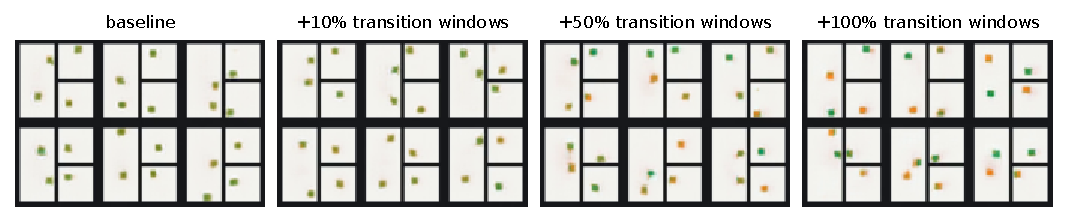
\includegraphics[width=\linewidth]{figures/lewm_transition_diversity_decoder.pdf}
  \caption{\textbf{Transition-focused sampling changes decoder appearance.}
  Selected reconstructions appear more saturated, but frames differ across
  conditions and cue identity is not measured. Coordinate $R^2$ does not
  improve consistently; added windows increase compute.}
  \label{fig:diversity}
\end{figure}

\FloatBarrier
\section{Additional readout diagnostics}
\label{app:diagnostics}

\begin{figure}[h]
  \centering
  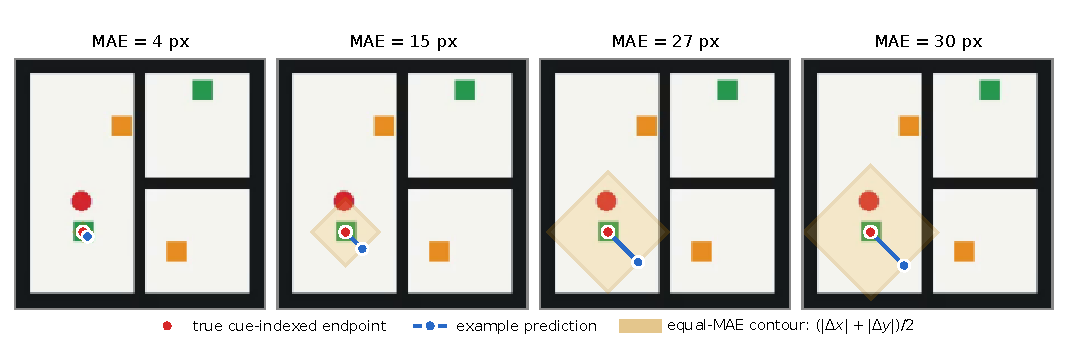
\includegraphics[width=.80\linewidth]{figures/tr2_color_mae_scale.pdf}
  \caption{\textbf{Coordinate error at the task scale.} The gold contour
  marks predictions with a fixed per-coordinate MAE; the blue point is one
  illustrative prediction. From left to right, the panels show 4 px
  (approximately the spatial Color location error), 15 px (a coarse-error
  example), 27 px (approximately the cue-coordinate error), and 30 px
  (an illustrative constant-baseline error). The task-specific constant baseline and
  $R^2$, not a universal pixel threshold, determine the interpretation.}
  \label{fig:mae}
\end{figure}

\paragraph{Visible hue remains accessible in patch tokens.}
A separate binary hue-classification audit of a historical Color+IDM checkpoint
achieves 100\% balanced accuracy from native patch tokens but 45.3\% from the
projected state (chance 50\%), using an episode-disjoint validation split.
This contrast localizes an accessibility gap along the compact-state
processing path; it does not establish an inability to perceive color.
Differences in feature dimensionality and readout capacity also preclude a
direct claim of information loss.

The hue classifier asks which hue occupies a portal slot; the coordinate
probe asks where a cue-indexed endpoint lies. The hue audit fits on 525
episodes, selects the ridge penalty using 75 validation episodes, and tests
on 150 episodes. The 640/256 coordinate protocol instead fixes the penalty.
Both readouts can miss information outside their chosen function class.
Likewise, MSE decoding can average uncertain outputs: its population optimum
is $d^*(z)=\mathbb E[X\mid z]$, but the representation, decoder capacity, and
optimization can limit the trained decoder.


\FloatBarrier
\section{Nonlinear probes}
\label{app:nonlinear}

Weak linear recovery does not imply that a representation lacks the target
information. LeWM's original study also uses nonlinear probes to assess
physical quantities \citep{maes2026leworldmodel}. We therefore fit a small MLP
to the same frozen states and endpoint targets used in the main paper.
The network has two 256-unit ReLU hidden layers and jointly predicts the
16 coordinates of the four positional and four cue-indexed endpoints.

We use 512 fit episodes, 128 validation episodes, and 256 episodes held out from probe
fitting. Feature and coordinate normalization use only the fit episodes.
For each of three probe initialization seeds, validation error selects the
learning rate ($10^{-3}$ or $3\times10^{-4}$), AdamW weight decay (0 or .01),
and stopping epoch. Training uses full batches of 512, at most 1,000 epochs,
and a patience of 100 epochs. Selection minimizes the mean squared error of
standardized coordinates across all targets. A ridge comparator uses the
same fit/validation split and selects its penalty from
$\{.01,.1,1,10,100,1000\}$; all six state/variant combinations select 100.
Test results are evaluated after these choices are fixed.

\begin{table}[!htbp]
\centering
\caption{\textbf{A small nonlinear probe leaves the location--cue gap largely intact.}
Metrics average four endpoints. MLP entries show mean $\pm$ sample SD
across three probe initializations, not world-model training runs. Both
methods fit 512 episodes; the main paper's fixed-penalty ridge uses 640.}
\label{tab:nonlinear}
\renewcommand{\arraystretch}{1.12}
\setlength{\tabcolsep}{3pt}
\begin{tabular*}{\linewidth}{@{\extracolsep{\fill}}llrrrr@{}}
\toprule
Variant & Probe & Cue MAE $\downarrow$ & Cue $R^2\uparrow$ & Location MAE $\downarrow$ & Location $R^2\uparrow$ \\
\midrule
\multicolumn{6}{l}{\emph{Current projected states}} \\
Color & Ridge & $27.48$ & $.262$ & $4.05$ & $.923$ \\
Color & MLP & $27.50\pm0.03$ & $.273\pm.005$ & $5.09\pm0.16$ & $.885\pm.006$ \\
Shape & Ridge & $27.91$ & $.250$ & $4.85$ & $.894$ \\
Shape & MLP & $27.74\pm0.07$ & $.261\pm.006$ & $5.76\pm0.13$ & $.857\pm.003$ \\
Palette & Ridge & $27.43$ & $.271$ & $4.24$ & $.913$ \\
Palette & MLP & $27.78\pm0.12$ & $.259\pm.003$ & $5.32\pm0.14$ & $.874\pm.005$ \\
\midrule
\multicolumn{6}{l}{\emph{One-step predicted states}} \\
Color & Ridge & $27.42$ & $.267$ & $3.92$ & $.926$ \\
Color & MLP & $27.53\pm0.06$ & $.273\pm.004$ & $5.03\pm0.14$ & $.887\pm.007$ \\
Shape & Ridge & $27.83$ & $.258$ & $4.72$ & $.900$ \\
Shape & MLP & $27.73\pm0.10$ & $.262\pm.005$ & $5.61\pm0.15$ & $.864\pm.004$ \\
Palette & Ridge & $27.58$ & $.270$ & $4.04$ & $.919$ \\
Palette & MLP & $27.80\pm0.14$ & $.260\pm.001$ & $5.18\pm0.18$ & $.881\pm.006$ \\
\bottomrule
\end{tabular*}
\end{table}

The MLP reaches cue $R^2=.259$--$.273$ for current states, while location
$R^2$ remains much higher at $.857$--$.885$ (Table~\ref{tab:nonlinear}). Its cue
scores are close to the validation-selected ridge baseline, and its location
scores are lower. The same pattern holds for predicted states. Within this
probe family and label budget, adding nonlinearity does not close the gap.
Larger probes or more labeled episodes could give different results; these
tests do not establish information loss.

\section{Controlled portal swaps and predicted crossings}
\label{app:portal-swap}

We exchange the two central-room portal endpoints to separate encoder
sensitivity from prediction of their consequences. Unordered locations stay
fixed, while visible identities and the destination reached from each entrance
switch together. Destination-room endpoints remain unchanged. Both worlds
are physically coherent: the intervention changes visible cues along with routing.

We use 16 planning geometries, eight per rank, with identical geometry and
actions across renderings. Figure~\ref{fig:swap-states} illustrates a separate
training geometry, excluded from all aggregates. Controls translate either
the agent or both central-room endpoints by eight pixels; the latter changes
occupied geometry while preserving identities. We measure squared projected-state
distance from the original observation, with same-state distance as a zero
reference.

\begin{figure}[!htbp]
\centering
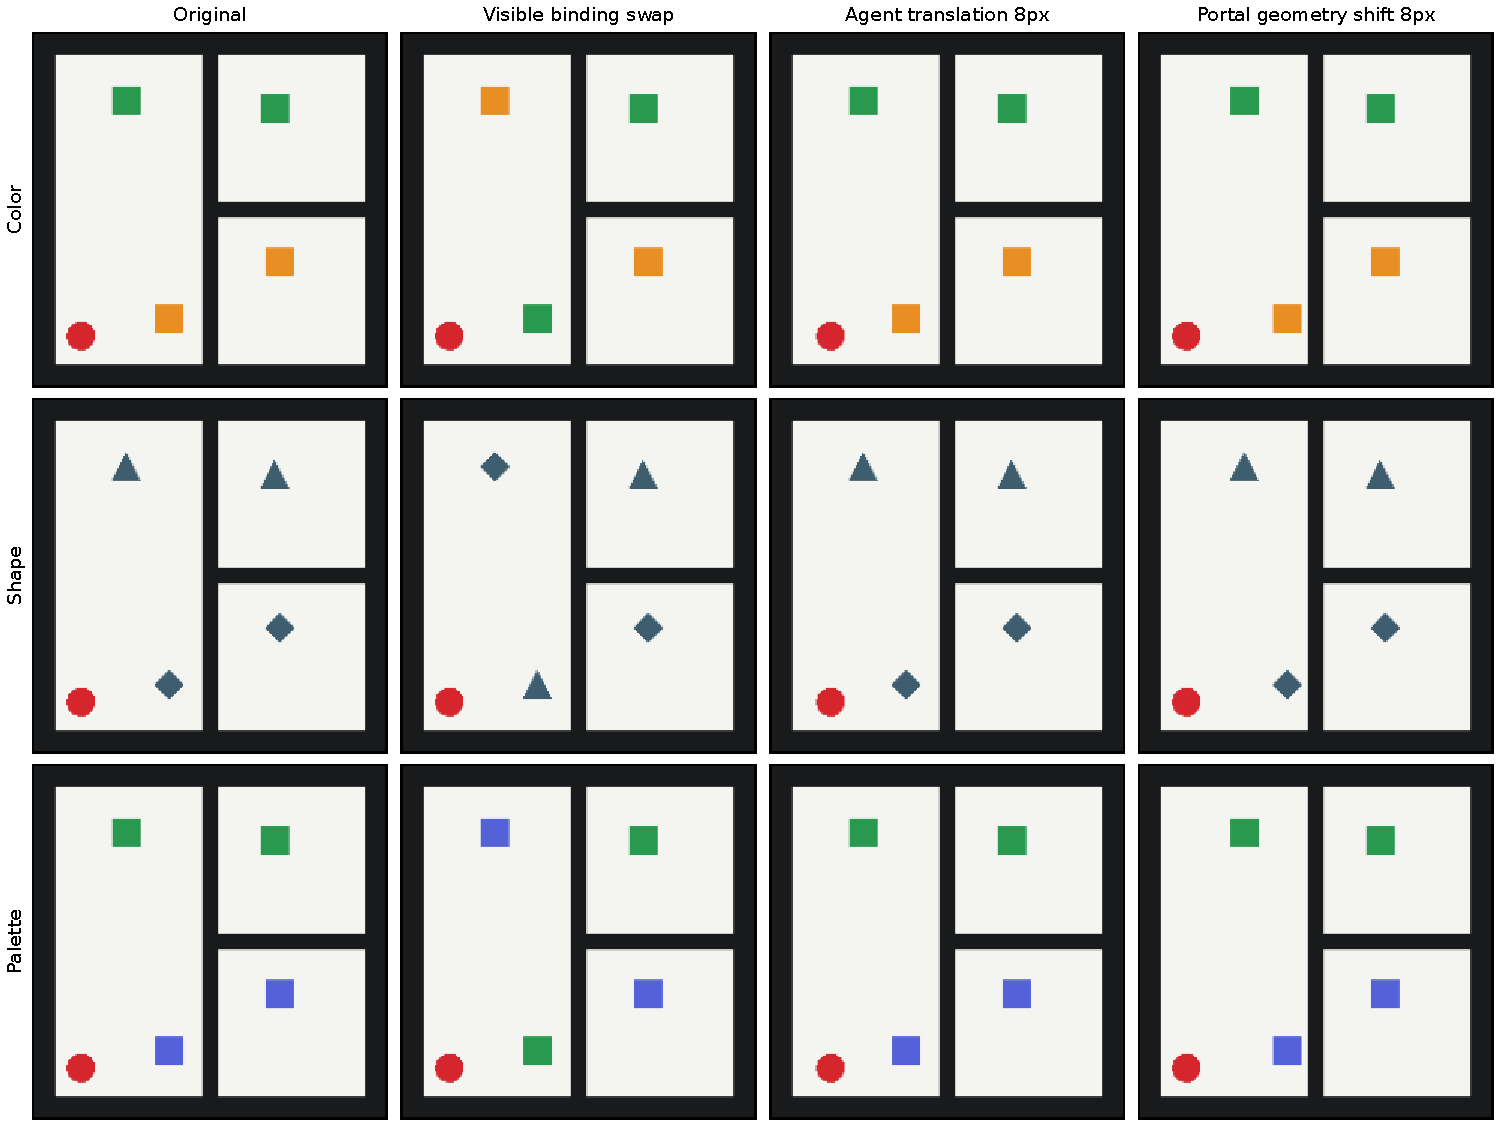
\includegraphics[width=\linewidth]{figures/lewm_portal_swap_states.pdf}
\caption{\textbf{Swapping visible cues changes where the same entrance leads.}
Original worlds, cue swaps, and eight-pixel translations of the agent or
central-room portals, for all three renderings of one illustration geometry.
The swap preserves occupied portal locations and destination-room cues.}
\label{fig:swap-states}
\end{figure}

For the dynamic comparison, each pair receives the same 80 primitive
actions: ten stationary steps, a straight approach to the nearer entrance,
and then zero actions. Both agents remain at identical positions until they
enter that physical portal, at the same step between 15 and 25, then arrive
in different destination rooms. Model forecasts start from observations at
steps 0, 5, and 10, all before the crossing. Subsequent states are predicted
autoregressively using the same normalized five-action blocks in both worlds;
observed post-crossing states are never fed back. We separately encode the
actual trajectories for comparison.

We plot squared distance between the two worlds' projected states and
between their two predicted states. Time zero is the first sampled frame at
or after the true crossing, so the event lies within the preceding five-step
interval. Figure~\ref{fig:swap-curves} shows raw within-model distances and
actual position separation; curves are medians with interquartile bands over
the 16 evaluation geometries.

\begin{figure}[!htbp]
\centering
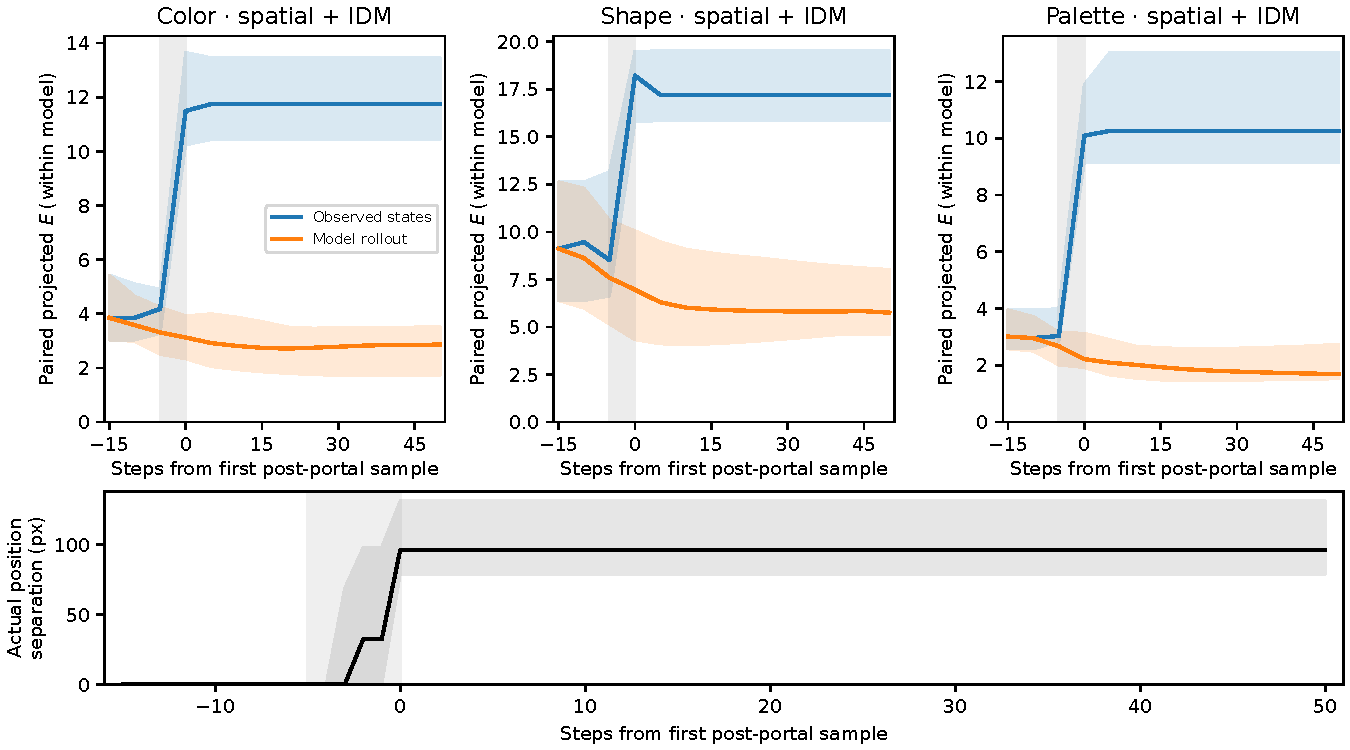
\includegraphics[width=\linewidth]{figures/lewm_portal_swap_raw_event_curves.pdf}
\caption{\textbf{Observed trajectories diverge at the portal; predictions understate the change.}
Top: paired squared latent distances for actual observations (blue) and
open-loop predictions (orange). Bottom: actual position separation, shared
across renderings. Medians and interquartile bands summarize 16 geometries.
The gray interval contains the first portal transition. Latent scales are
interpreted within each model, not across columns.}
\label{fig:swap-curves}
\end{figure}

\begin{table}[!htbp]
\centering
\caption{\textbf{Cue swaps are detectable, but their predicted consequences are attenuated.}
Static ratios use each case's agent-shift energy. The forecast ratio compares
mean predicted and observed separation over the first three post-crossing
samples. Entries show medians [25th, 75th percentiles] across 16 geometries,
not confidence intervals.}
\label{tab:swap}
\renewcommand{\arraystretch}{1.12}
\setlength{\tabcolsep}{4pt}
\begin{tabular*}{\linewidth}{@{\extracolsep{\fill}}lrrr@{}}
\toprule
Variant & Cue swap / agent shift & Portal shift / agent shift & Forecast / observed \\
\midrule
Color & 0.92 [0.71, 1.06] & 5.66 [3.99, 7.34] & 0.25 [0.17, 0.31] \\
Shape & 1.72 [1.16, 2.34] & 5.94 [4.42, 8.04] & 0.42 [0.30, 0.46] \\
Palette & 0.58 [0.39, 0.67] & 3.79 [3.27, 5.69] & 0.18 [0.15, 0.26] \\
\bottomrule
\end{tabular*}
\end{table}

Swaps elicit nonzero responses comparable to an eight-pixel agent shift
(Table~\ref{tab:swap}); the encoder is not cue invariant. Portal translation
produces larger median responses. After crossing, median forecast/observed
separation ratios are .25, .42, and .18 for Color, Shape, and Palette, with
attenuation in every evaluated pair. These rollouts understate the routing
change's consequences, but general prediction error or open-loop contraction
may contribute. A dynamic translation control would help distinguish these
explanations.


\FloatBarrier
\section{Related work and interpretation}
\label{app:related}

Predictive feature learning now spans several distinct settings. I-JEPA and
V-JEPA learn from masked image and video content
\citep{assran2023ijepa,bardes2024vjepa}; Image World Models study prediction
of photometric transformations and the roles of conditioning and predictor
capacity \citep{garrido2024iwm}. V-JEPA~2 connects video pretraining to
action-conditioned robot planning \citep{assran2025vjepa2}, while
V-JEPA~2.1 adds dense and intermediate-layer supervision to improve spatial
and temporal features \citep{murlabadia2026vjepa21}. These successes motivate
testing which task distinctions remain accessible after prediction in
feature space, especially when they occupy little of the image.

Latent planning can use either pretrained visual features or representations
learned jointly with dynamics. DINO-WM predicts spatial patch features from
a pretrained DINOv2 encoder \citep{zhou2025dinowm,oquab2023dinov2}.
PLDM learns predictive dynamics from reward-free offline interactions
\citep{sobal2025latentplanning}; LeWorldModel and LpWM study end-to-end
learning with different distribution regularizers
\citep{maes2026leworldmodel,kuang2026lpwm}. Our positive control belongs to
the latter line, with its particular recipe stated in
Appendix~\ref{app:planning}. Its stronger planning motivates a controlled
comparison of learned cue binding; it does not establish that sparsity alone
explains the difference.

Regularization and identifiability provide complementary perspectives.
VICReg explicitly controls feature variance and covariance
\citep{bardes2022vicreg}; LeJEPA studies isotropic Gaussian regularization
\citep{balestriero2025lejepa}, and Rectified LpJEPA develops sparse,
nonnegative alternatives \citep{kuang2026rectified}.
In \emph{When Does LeJEPA Learn a World Model?}, Klindt et al.
\citep{klindt2026when} establish linear recovery under assumptions including
independent Gaussian latent variables and stationary additive-noise
transitions. This is an encoder-side result under a specified data model,
not a general guarantee for an action-conditioned predictor. We do not
establish those assumptions for Tunnel Rooms, so our findings do not
contradict that theorem.

Feature selection can nevertheless favor the wrong information for a task.
Sobal et al. \citep{sobal2022slow} show that JEPAs can prefer stationary
noise over a moving object in controlled experiments. Littwin et al.
\citep{littwin2024jepa} analyze a bias toward more predictable features in
deep linear self-distillation networks. These results motivate examining
the relation between predictability and usefulness, but neither identifies
the cause of our cue-binding gap: our cues persist and determine destination
pairings. The transition-exposure experiment therefore tests a separate
possibility and remains inconclusive.

Additional training signals offer ways to align representations with action.
Sensorimotor World Models use inverse dynamics
\citep{ivashkov2026sensorimotor}; auxiliary-task theory explains how added
targets can preserve otherwise unresolved distinctions \citep{yu2025auxjepa}.
Value-guided JEPA planning explicitly aligns latent distance with a
goal-reaching value function \citep{destrade2025value}, while PSG-JEPA adds
training-time physical-state grounding \citep{yan2026psgjepa}.
Temporal Straightening regularizes latent trajectories for planning
\citep{wang2026temporal}; its learned feature aggregation inspires our
different spatial readout (Appendix~\ref{app:aggregator}). Together, these
directions motivate testing which additional constraints help retain cue
identity and destination, beyond improving average prediction or marker
visibility.


\end{document}
